% Template:     Auxiliar LaTeX
% Documento:    Archivo principal
% Versión:      8.3.3 (20/01/2025)
% Codificación: UTF-8
%
% Autor: Pablo Pizarro R.
%        pablo@ppizarror.com
%
% Manual template: [https://latex.ppizarror.com/auxiliares]
% Licencia MIT:    [https://opensource.org/licenses/MIT]

% CREACIÓN DEL DOCUMENTO
\documentclass[
	spanish, % Idioma: spanish, english, etc.
	letterpaper, oneside
]{article}

% INFORMACIÓN DEL DOCUMENTO
\def\documenttitle {Auxiliar 2}
\def\documentsubject {Coordenadas cilíndricas y esféricas}

\def\documentauthor {Nombre del autor}
\def\coursename {Mecanica}
\def\coursecode {FI-2001}

\def\universityname {Universidad de Chile}
\def\universityfaculty {Facultad de Ciencias Físicas y Matemáticas}
\def\universitydepartment {Departamento de la Física}
\def\universitydepartmentimage {departamentos/fcfm}
\def\universitydepartmentimagecfg {height=1.75cm}
\def\universitylocation {Santiago de Chile}

% EQUIPO DOCENTE
\def\teachingstaff {
	\textbf{Profesor: Simón Riquelme} \\
	Auxiliares: Jorge Barja, Ian Tobar \\
	Ayudante: Matías Abrigo  \\
}

% IMPORTACIÓN DEL TEMPLATE
\input{template}

% INICIO DE PÁGINAS
\begin{document}

% CONFIGURACIÓN DE PÁGINA Y ENCABEZADOS
\templatePagecfg

% ======================= INICIO DEL DOCUMENTO =======================

\newboxquestion{P1}\\

Considere una curva espiral descrita en coordenadas esféricas por las ecuaciones:
\begin{center}
$ r = R$ , $ \phi = N\theta $
\end{center}
donde R y N son constantes conocidas (N entero par). Una partícula se mueve sobre la espiral partiendo desde el extremo superior ($ \dot{\theta} = w_0 $). Se pide:

\begin{enumerate}[label=\alph*)]
    \item Utilizando coordenadas esféricas, escriba los vectores velocidad y aceleración para una posición arbitraria de la partícula sobre su trayectoria.
    \item Encuentre una expresión para la longitud total de la espiral y para el tiempo que la partícula tarda en recorrerla.

\end{enumerate}


\begin{figure}[h] % [h] indica que se coloca la imagen aquí (here)
    \centering % Centra la imagen
    
\includegraphics[width=0.4\textwidth]{p2.png} % Ajusta el tamaño de la imagen
    \caption{Pregunta 1.} % Subtítulo de la imagen
    \label{fig:p1} % Etiqueta opcional para referencias
\end{figure}

\newpage

\newboxquestion{P2}\\

Daniel está en un coliseo circular de radio $a$ y centro $O$ junto con un León que lo persigue. Daniel desea escapar del León, la estrategia que utiliza Daniel para arrancar es correr por el perímetro del coliseo con una rapidez $u$, mientras que el León corre con una rapidez $U$ moviéndose hacia Daniel, manteniéndose siempre en el radio $OD$. Inicialmente Daniel se encuentra en el borde del coliseo mientras que el León se encuentra en el centro $O$. La situación está descrita en la figura.

\begin{enumerate}[label=\alph*)]
    \item Muestre que $r$, la distancia $OL$ satisface la ecuación:
    $$ \dot{r}^2 = \frac{u^2}{a^2} \left ( \frac{U^2a^2}{u^2} - r^2\right) $$
    
    \item Encuentre $r$ en función del tiempo, $r(t)$.
    
    \item Muestre que si $U \geq u $ Daniel será atrapado y encuentre cuanto tardará que esto ocurra.

    \item Muestre que el León recorre un arco de circunferencia.

    \item Para el caso $U=u$, bosqueje el camino tomado por el León y encuentre el punto de captura (propuesto).
\end{enumerate}

\begin{figure}[h] % [h] indica que se coloca la imagen aquí (here)
    \centering % Centra la imagen
    \hspace{-1.5cm} % Desplaza la imagen 2 cm a la izquierda
    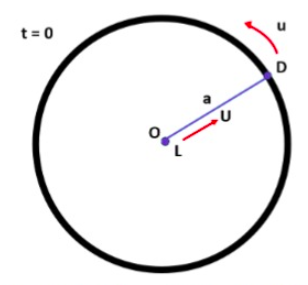
\includegraphics[width=0.3\textwidth]{p2.2.png} % Ajusta el tamaño de la imagen
    \caption{Pregunta 2.} % Subtítulo de la imagen
    \label{fig:p2} % Etiqueta opcional para referencias
\end{figure}

% \newboxquestion{P2}\\

% Una partícula se mueve a lo largo de una trayectoria espiral cilíndrica (ver figura) con una rapidez v(t). La distancia desde cualquier punto de la trayectoria al eje del espiral es R y el angulo que forma el vector velocidad con el plano perpendicular al eje del espiral ($ \alpha $) es constante. Determine en términos de R, v(t) y $ \alpha $ la velocidad y aceleración en cilíndricas. 

% \begin{figure}[h] % [h] indica que se coloca la imagen aquí (here)
%     \centering % Centra la imagen
%     \hspace{-1.5cm} % Desplaza la imagen 2 cm a la izquierda
%     
\includegraphics[width=0.4\textwidth]{p1.png} % Ajusta el tamaño de la imagen
%     \caption{Pregunta 2.} % Subtítulo de la imagen
%     \label{fig:p2} % Etiqueta opcional para referencias
% \end{figure}

\newboxquestion{P3} ($\star$) \\

Una partícula se mueve con rapidez v$_0$ constante, sobre un riel circular de radio R colocado en posición horizontal sobre una superficie también horizontal. La partícula se encuentra atada mediante una cuerda inextensible a un bloque que cuelga debajo de un agujero localizado a una distancia R/2 del centro del riel. Suponga que v$_0$ es suficientemente pequeño para que la cuerda no se destense.

\begin{enumerate}[label=\alph*)]
    \item Determine la rapidez del bloque en función del ángulo $\theta$.
    %Sol: $ v(\theta) = \frac{\sin\theta}{\sqrt{5 + 4\cos \theta}}v_0 $
    \item Obtenga la rapidez máxima del bloque.
    %Sol: $ \vec{v}_{max} = \pm \frac{v_0}{2} \hat{k}$
    \item Determine la aceleración $\vec{a}$ del bloque cuando la partícula que se mueve sobre el riel pasa por la posición $\theta$ = 0 (propuesto).
    %Sol: $ \vec{a}(\theta = 0) = - \frac{v^2_0}{3R} \hat{k}$
\end{enumerate}

\begin{figure}[h!] % [h] indica que se coloca la imagen aquí (here)
    \centering % Centra la imagen
    \includegraphics[width=0.5\textwidth]{Pa.png} % Ajusta el tamaño de la imagen
    \caption{Pregunta 3.} % Subtítulo de la imagen
    \label{fig:p3} % Etiqueta opcional para referencias
\end{figure}



\newboxquestion{P4} (\textbf{Propuesto $\star$}) \\

El punto de unión P entre un pistón y una biela de largo D se mueve a lo largo del eje x debido a que el cigüeñal (disco), de radio R y centro en un punto fijo O, rota a una velocidad angular constante w.
En el instante t = 0 la biela está horizontal ($\phi$ = 0, x = R + D).

\begin{enumerate}[label=\alph*)]
    \item Encuentre una expresión para la distancia x(t) entre P y O como función del tiempo.\\
    Sol: $ x(t) = R\cos(wt) + \sqrt{D^2 - R^2 \sin^2(wt)} $
    \item Encuentre la velocidad v(t) de P.\\
    Sol: $ v(t) = -Rw\sin(wt)[1 + \frac{R\cos(wt)}{\sqrt{D^2 - R^2 \sin^2(wt)}}] $
    \item En la expresión para la v(t) considere el caso R $ \ll $ D y luego encuentre una expresión aproximada para la aceleración de P. ¿Cómo se compara la magnitud de la aceleración máxima del pistón con la aceleración del punto A?.\\
    Sol: $ v(t) \approx -Rw \sin(wt) ; a(t) \approx -Rw^2\cos(wt) $
\end{enumerate}

\begin{figure}[h] % [h] indica que se coloca la imagen aquí (here)
    \centering % Centra la imagen
    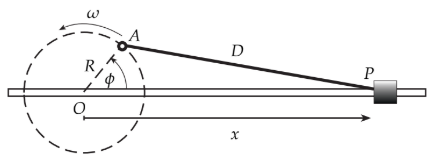
\includegraphics[width=0.5\textwidth]{p5.png} % Ajusta el tamaño de la imagen
    \caption{Pregunta 4.} % Subtítulo de la imagen
    \label{fig:p4} % Etiqueta opcional para referencias
\end{figure}

% FIN DEL DOCUMENTO
\end{document}